\chapter{Squiggles Alignment}

\label{kap:squiggles} % id kapitoly pre prikaz ref

In this chapter, we describe our work. We took a different approach to composing DNA sequence from multiple squiggles. 
We took squiggles that correspond to the same part of the reference sequence and aligned them together to produce one signal that will be basecalled. We designed several ways of multiple squiggles alignment to generate signal most similar to the ideal signal.

\section{Squiggles and preprocessing}

The MinION device produces sequences of measured values of current passing nanopores. We call this sequences squiggles.
Typically we have multiple squiggles covering each part of the DNA. Raw signal contain values in pA between $0$ and several hundred. 
This values have a consistent deviation in single read but can be shifted in different read from different nanopore. 

The best way to hide this differences is to scale the sequence such that resulting mean value is 0 and a standard deviation is 1 
\cite{kubo}.

\section{Squiggles alignment with Dynamic Time Warping}
To align two squiggles we use the method called Dynamic Time Warping (DTW).
DTW is widely used in audio processing and speech recognition \cite{muller2007dynamic}.
It uses a similar approach as the Needleman-Wunsch algorithm for sequence alignment but 
does not specify score of match or mismatch but cost function for any pair of values.

\subsection{Dynamic Time Warping}

We define a cost function $c(i,j)$ which tells us price for aligning value $i$ to value $j$. 
It can be for example euclidean distance $abs(i-j)$.

By evaluating cost function for two sequences $u$ and $v$, we calculate a cost matrix $C$ where $C[i,j] = c(u_i,v_j)$.
The best alignment of this two sequences can be represented as a continuous path from $C[1,1]$ to $C[n,m]$ with the lowest sum of costs (Fig. \ref{fig:wp}). 
We call such path a warping path and sum of costs a cost of alignment. The cost of alignment also tells us the similarity of those sequences.


\begin{figure}[h]
  \centering
  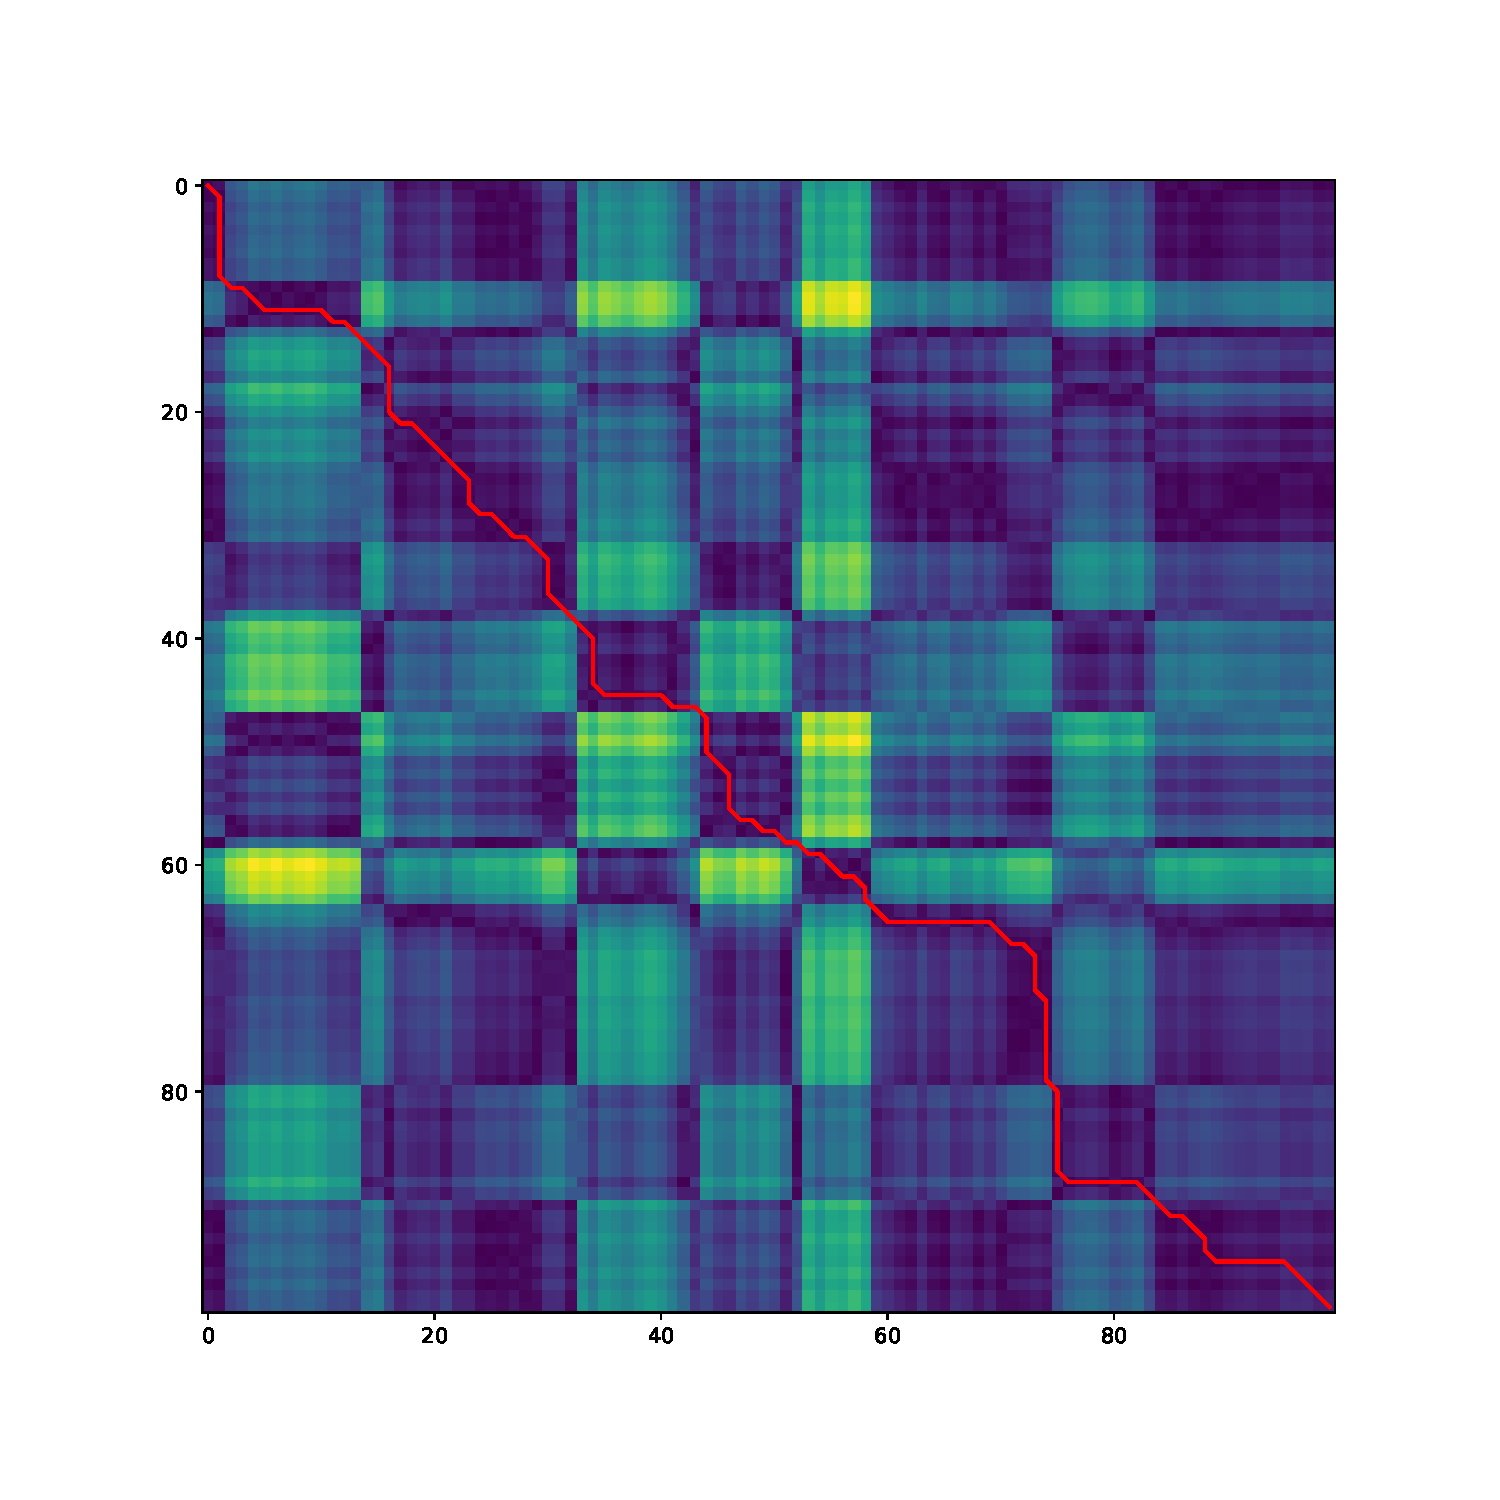
\includegraphics[width=0.8\textwidth]{images/wp}
  \caption{Warping path in matrix $C$.}
  \label{fig:wp}
\end{figure}

The warping path can be represented as a list of coordinates from matrix $C$.

\subsection{Implementation}
To find the best path, we will not compute matrix $C$ with costs of aligning single values.
Instead, we will calculate matrix $A$ where $A[i,j]$ contains cost of alignment of sequences $u_1 \dots u_i$ and $v_1 \dots v_j$, 
same as we did in Needleman-Wunsh algorithm.

$A[i,j]$ will be computed as $min(a[i-1,j],a[i,j-1],a[i-1,j-1])+c(i,j)$. 

Finally, we will find warping path in $A$ by following lowest values from $A[n,m]$ to $A[1,1]$. 

The complexity of this implementation is quadratic but can be simply reduced to almost linear by restricting area where the warping path can be to a band with a constant width (Fig. \ref{fig:belt}). We will define $c(i,j)=\infty$ for all $i,j$ not in the belt. This way the values that are not computed will not affect final value. By checking the coordinates of a chosen point while constructing warping path, we can find out if chosen belt covers whole warping path. 
When the belt is not wide enough, we will restart computation with a twice as wide belt.
\begin{figure}[h]
  \centering
  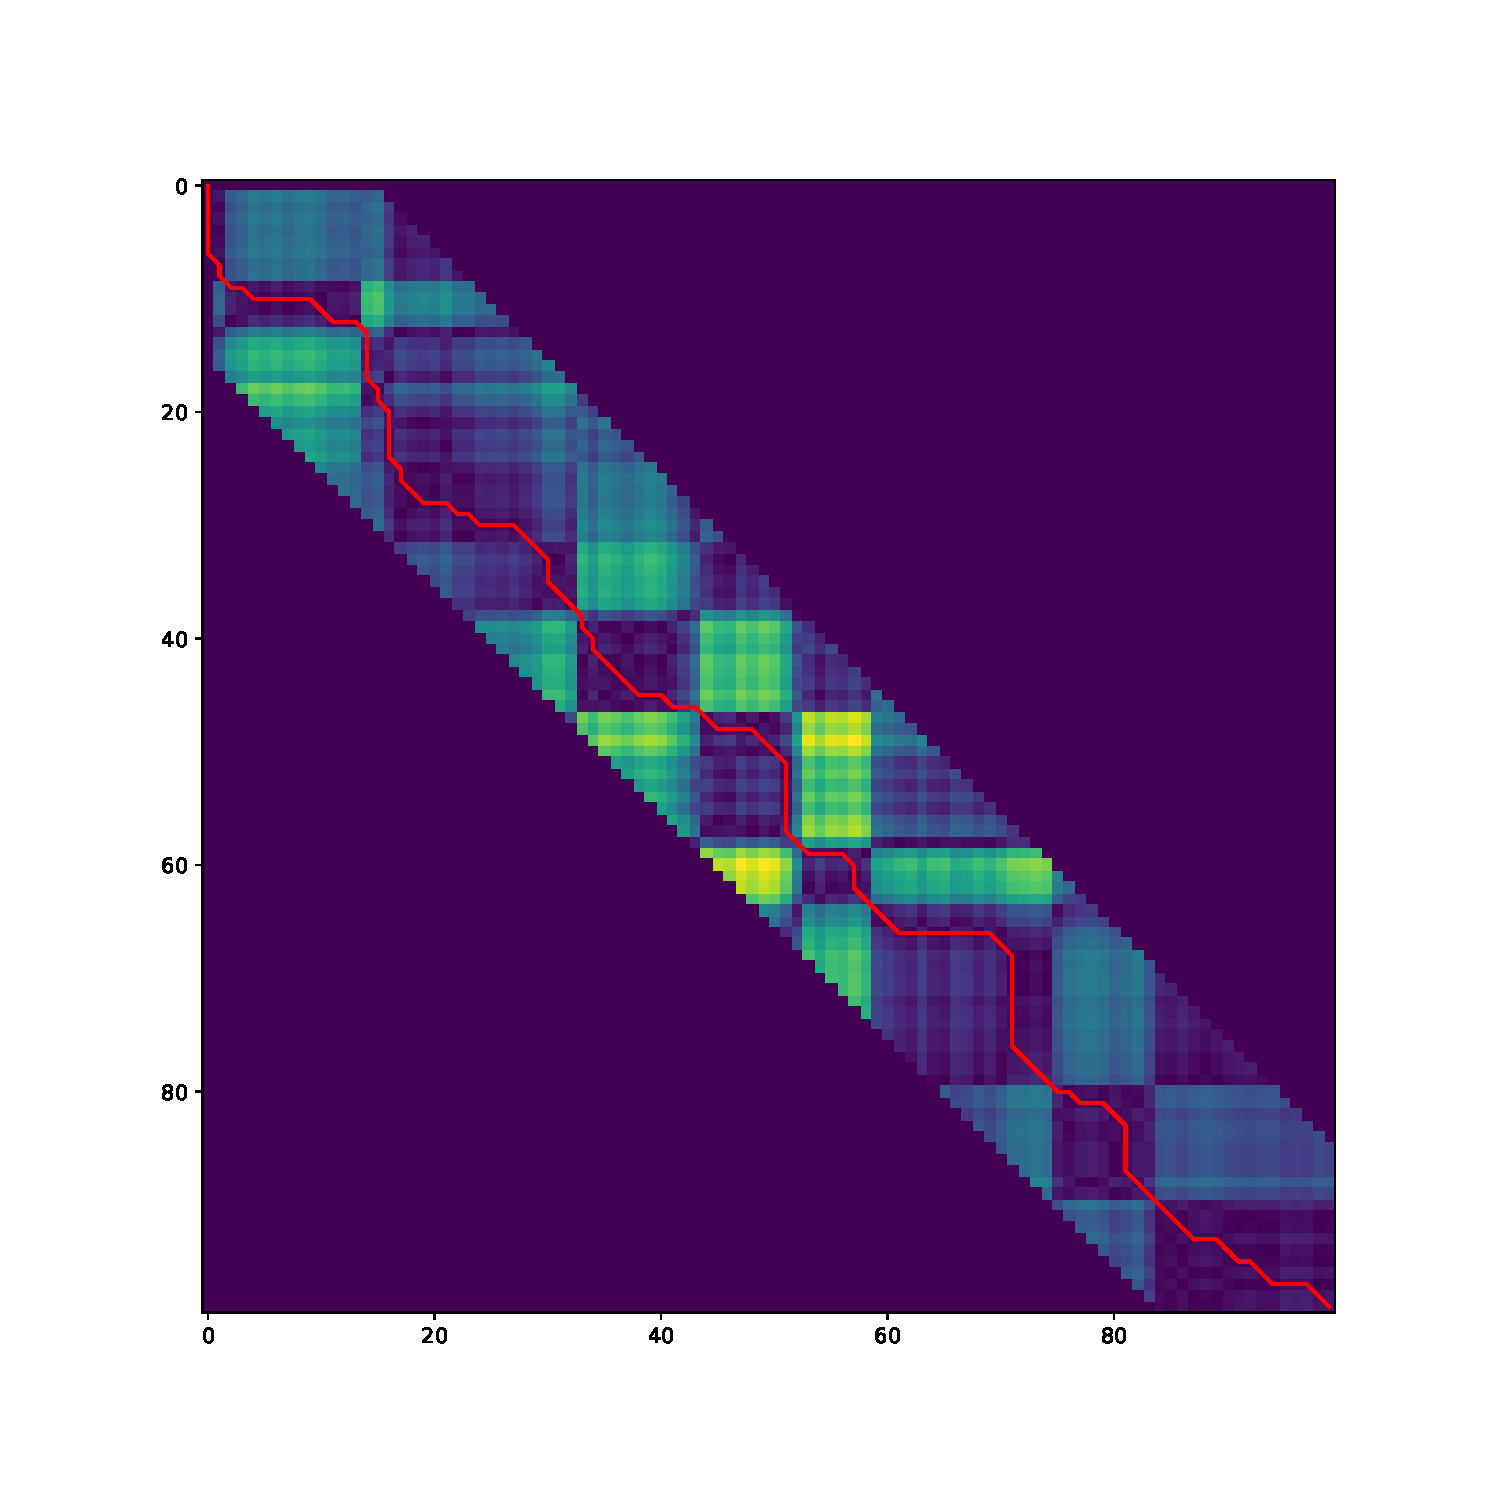
\includegraphics[width=0.8\textwidth]{images/wp2}
  \caption{Belt restricted warping path in matrix $C$.}
  \label{fig:belt}
\end{figure}


\subsection{Signal reconstruction from warping path}

To create one signal out of two, we will use the warping path created by DTW.
Although the signals are very similar, alignment still contains some insertions in both ways (Fig. \ref{fig:pairing}). 
\begin{figure}
  \centering
  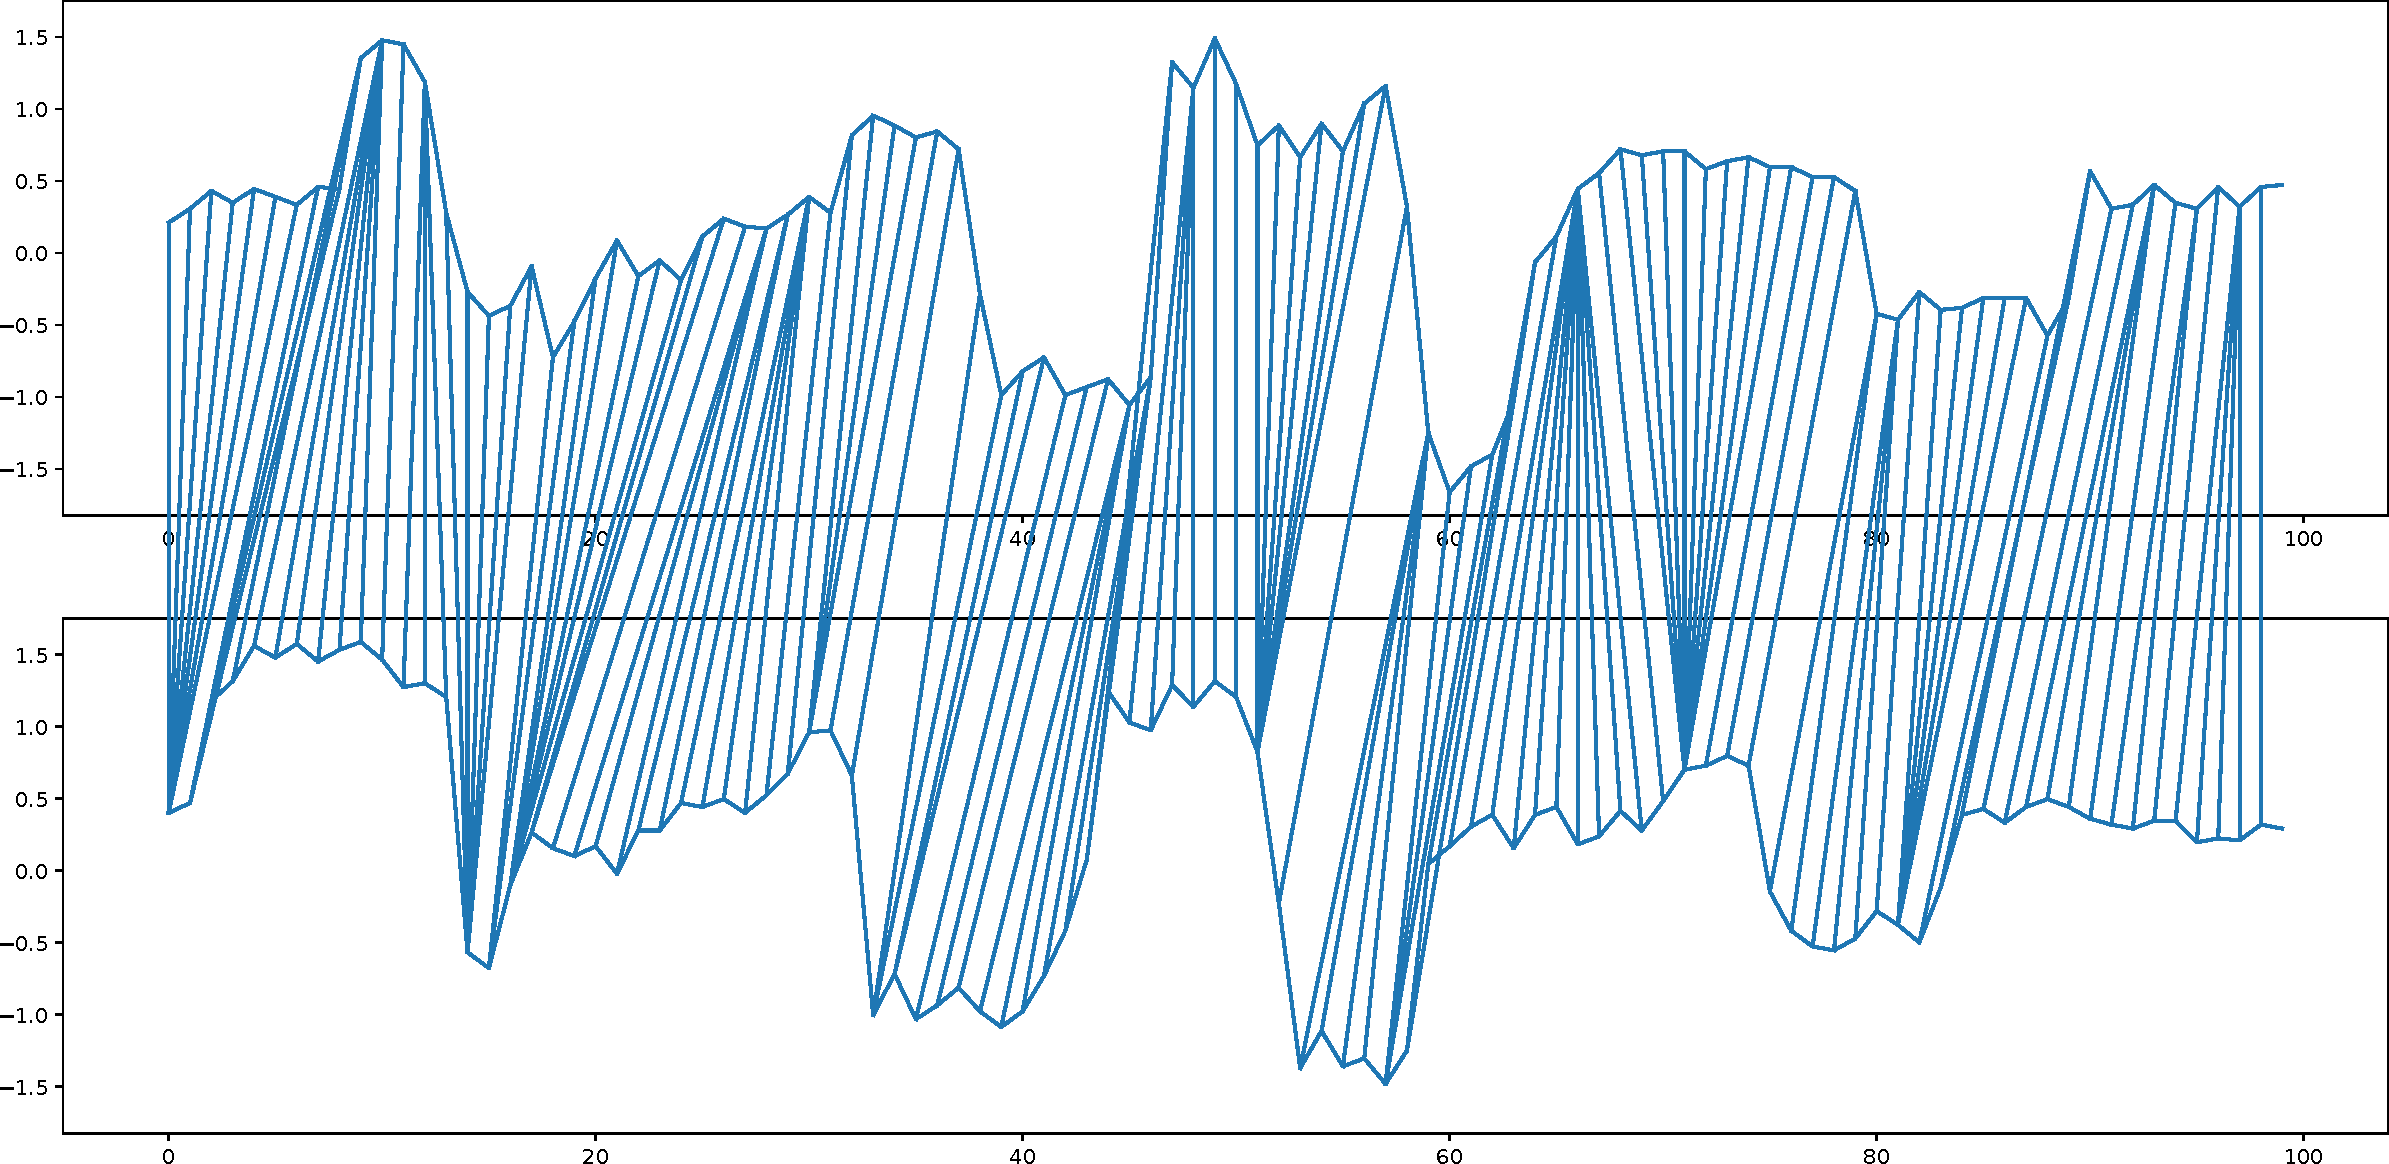
\includegraphics[width=1.0\textwidth]{images/ciary}
  \caption{Pairing of points created by DTW.}
  \label{fig:pairing}
\end{figure}

When aligning DNA sequences, we had three possibilities. Match, mismatch or aligned to dash. 
This time, we have a pairing of points. Each point from the first sequence have the corresponding point
in the second sequence and each point from the second sequence have the corresponding point
in the first sequence. This also means, that sometimes one point from one sequence corresponds to multiple points from the other sequence.

We considered multiple ways to solve this problem.

The first approach is to calculate an average of each pair of points and concatenate them to final signal. The signal we created
was slightly longer.

The second approach is to take the first sequence as leading and construct final signal by calculating an average of a point from this sequence and all points aligned to it, in every point of this sequence. 
This approach puts a high weight to the first sequence.

If some part of the signal from the second sequence is missing in the first sequence, it will still miss.
Same if some part of the first signal is longer than should, one point from the second signal will align to it, and it will stay there.
An advantage of this approach is, that the resulting signal looks exactly like a signal that basecaller expect.

\subsection{Multiple alignment}

To align multiple signals, we chosen the iterative method as signals are much longer than DNA sequences and iterative method is faster.

If we would just add sequences one by one and each time generates a resulting signal, weight of each next added signal will be higher.
We have tried multiple approaches to solve this problem.

The first approach was to calculate weighted average when aligning $i$-th signal to the consensus of $i-1$ already aligned signals. 
The result is that at each point, every sequence has the same weight in consensus.

The second approach was an improvement of the first one, by remembering how many points were aligned from all sequences to each point of consensus. We used
this information when reconstructing the final signal. For each point, we calculated an average number of point aligned to it and put it that many times to final sequence.

With this different way of reconstructing final sequence, we can afford to take full alignment each time. 
It will result in much longer signal than expected, which will be later reduced by realigning all sequences to it and counting 
points aligned to each point in it.